%07/10 - Blanca Lizarbe
\chapter{Aplicaciones del Procesamiento Digital de Imágenes: CT, PET \& SPECT, Ultrasonido y Microscopía}
\section{Introducción y relación con la MRI}

La resonancia magnética (MRI) utiliza campos magnéticos y pulsos de radiofrecuencia, produciendo imágenes de tejidos blandos con alto contraste. Al igual que la MRI, la tomografía computarizada (CT) y la tomografía por emisión de positrones (PET) emplean reconstrucción tomográfica (a partir de información 2D se genera información 3D), aunque con diferentes fundamentos físicos y datos. Comprender los principios físicos de cada modalidad ayuda a anticipar los desafíos del procesamiento digital de imágenes. Una pregunta relevante sería: ¿qué características de las imágenes en el procesamiento de MRI se compartirán o diferirán en CT o PET? Todas son imágenes que se toman in vivo de todo el cuerpo. En cuanto al procesamiento, todos tienen el problema del movimiento, teniendo que corregir los artefactos de movimiento. PET tiene una resolución espacial más grande, por lo que el movimiento puede notarse menos, pero sigue afectando. En resonancia, hay un sesgo por el campo no ajustado. Los tipos de sensores que utilizan CT y PET tienen que sentir una radiación, teniendo otro tipo de sensibilidad.

\section{Tomografía Computarizada (CT/TAC)}

La CT utiliza una fuente de rayos X que rota alrededor del paciente, y los detectores miden la atenuación de los rayos X al atravesar los tejidos. Cada píxel de la imagen corresponde a una unidad de Hounsfield (HU) que representa la densidad del tejido.

En cuanto a las técnicas de reconstrucción, la retroproyección filtrada (FBP) aplica la transformada de Radon inversa para reconstruir la imagen a partir de proyecciones, mientras que los métodos iterativos mejoran el control del ruido y los artefactos, especialmente en exploraciones de baja dosis.

\begin{figure}[h]
\centering
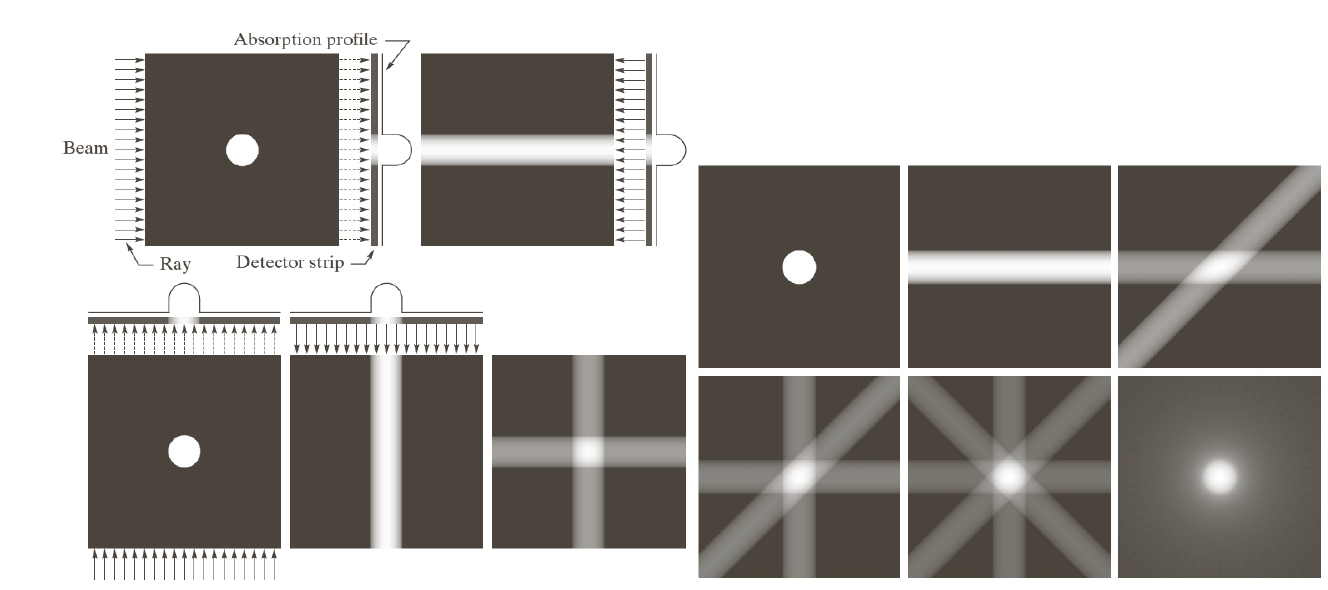
\includegraphics[width = 0.8\textwidth]{figs/backprojection.png}
\end{figure}

Las imágenes de CT presentan un alto contraste entre hueso y tejido blando, pero suelen ser más ruidosas que las de MRI. Los artefactos más comunes incluyen el \textbf{endurecimiento del haz} o \textit{beam hardening}, la dispersión y los artefactos metálicos. El endurecimiento del haz ocurre cuando los rayos X de menor energía son absorbidos preferentemente por estructuras densas, como hueso o implantes metálicos, lo que altera la interpretación del detector y genera efectos como bandas o “oscurecimiento” central. 

\begin{figure}[h]
\centering
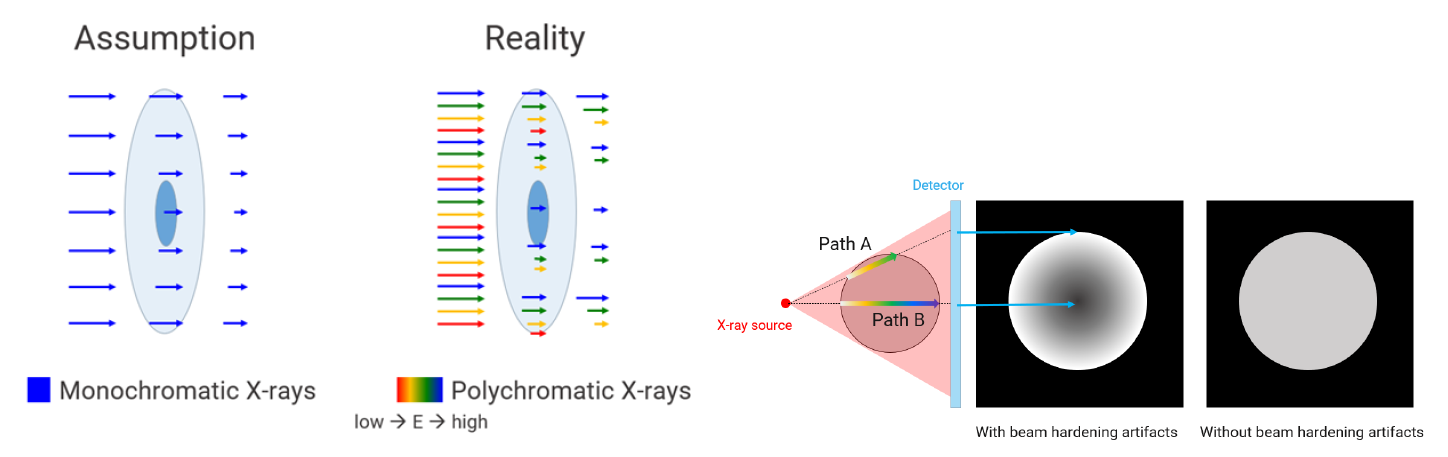
\includegraphics[width = \textwidth]{figs/beam-hardening.png}
\caption{La longitud del camino es corto para el camino A y largo para el B. Esto hace que haya menos endurecimiento del haz en el camino A y poca energía resultante de rayos X, además de alta tasa de absorción calculada y alta densidad reconstruida (claro). El camino B tiene más endurecimiento, mucha energía de rayos X, poco ratio de absorción calculado y poca densidad (oscuro).}
\end{figure}

La \textbf{dispersión}, causada principalmente por el efecto Compton, desvía los rayos X de su trayectoria, reduciendo el contraste y aumentando el ruido. Finalmente, los \textbf{artefactos metálicos} aparecen como bandas brillantes u oscuras alrededor de implantes metálicos.

El procesamiento de imágenes CT requiere preprocesamiento cuidadoso, reducción de ruido y artefactos. La segmentación enfrenta dificultades para diferenciar tejidos blandos y patológicos, y los datos volumétricos 3D exigen algoritmos eficientes para renderizado y análisis. Clínicamente, la CT se usa ampliamente en traumatismos, enfermedades pulmonares y óseas, y guía la planificación quirúrgica o de radioterapia. La física de la atenuación de rayos X influye directamente en los tipos de ruido y artefactos esperados.

\section{PET y SPECT}

La PET utiliza trazadores radiactivos que emiten positrones; estos se aniquilan con electrones, produciendo dos fotones de 511 keV detectados de forma coincidente por un anillo de detectores, permitiendo la reconstrucción tomográfica de la distribución del trazador, que refleja actividad metabólica o molecular. La SPECT, en cambio, usa trazadores que emiten fotones gamma simples, capturados mediante una cámara gamma que rota alrededor del paciente. Trazadores comunes incluyen Tecnecio-99m o Yodo-123. Las proyecciones obtenidas se reconstruyen en mapas tridimensionales mediante retroproyección filtrada o métodos iterativos.

La PET alcanza generalmente mayor sensibilidad y mejor resolución espacial que la SPECT, la cual está limitada por las estadísticas de fotones y la eficiencia del colimador. Ambas modalidades presentan un ruido considerable y baja resolución comparadas con CT o MRI, requiriendo algoritmos avanzados de corrección y eliminación de ruido. Las técnicas de aprendizaje profundo se aplican cada vez más para la mejora y reconstrucción de imágenes.

Debido al bajo conteo de fotones, las imágenes PET y SPECT suelen ser ruidosas, siendo SPECT la más afectada. La corrección por atenuación y dispersión es más compleja en SPECT, ya que depende de la emisión de fotones individuales y de la atenuación variable según los tejidos. Las imágenes PET y SPECT suelen fusionarse con exploraciones anatómicas (CT o MRI), lo que exige algoritmos de registro precisos para evitar desalineaciones que afecten la interpretación clínica. La segmentación y cuantificación presentan desafíos adicionales, como la definición precisa de regiones y la compensación de factores físicos y fisiológicos.

\begin{figure}[h]
\centering
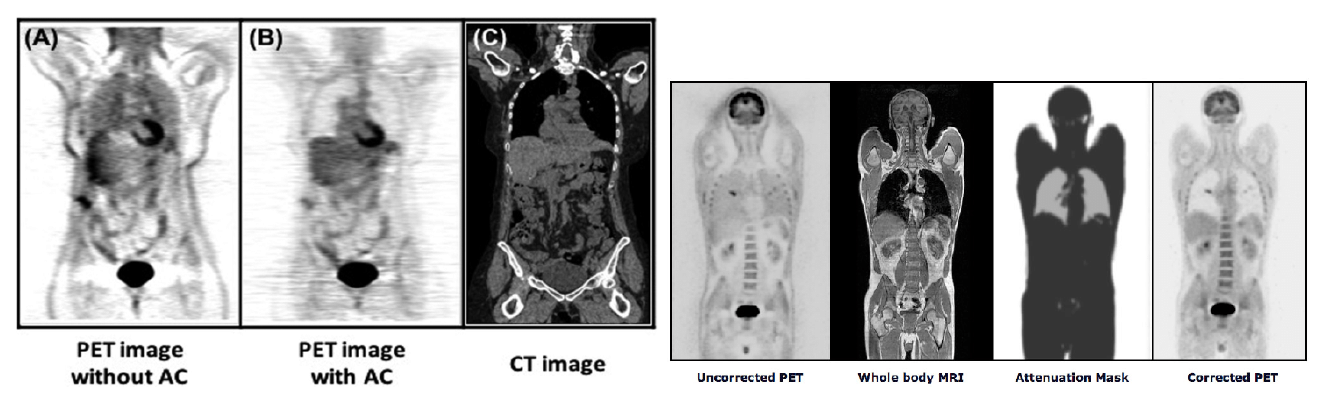
\includegraphics[width = \textwidth]{figs/atenuation-correction.png}
\caption{Corrección de atenuación (AC por sus siglas en inglés): A medida que los fotones emitidos por el trazador radiactivo viajan a través del cuerpo, algunos fotones son absorbidos o dispersados por tejidos como huesos, músculos o grasa. Esta pérdida de fotones significa que los detectores reciben menos fotones de los tejidos más profundos o densos, lo que hace que estas regiones parezcan artificialmente menos activas en las imágenes PET o SPECT.}
\end{figure}

En la práctica clínica, la PET se usa en oncología (detección y estadiaje tumoral), neurología (metabolismo cerebral) y cardiología (perfusión miocárdica). La SPECT se aplica en estudios de perfusión cardíaca, imagen ósea y cerebral, mapeo de receptores y diagnóstico de infecciones o inflamación. Aunque la resolución espacial es menor y tenga más artefactos y desventajas, su bajo costo y amplia disponibilidad de trazadores la hacen muy utilizada.

\section{Ultrasonido}

La ecografía utiliza ondas sonoras de alta frecuencia emitidas por un transductor, un dispositivo con un material que vibra con la electricidad para generar las ondas. Estas ondas viajan a través de los tejidos y se reflejan en las interfaces, siendo luego captadas y reconstruidas en imágenes en tiempo real. El proceso es altamente dependiente del operador y de las propiedades del tejido.

Uno de los principales desafíos del procesamiento de imágenes ecográficas es el ruido de moteado (\textit{speckle}), que surge por interferencia coherente de las ondas y genera un aspecto granular que reduce el contraste y dificulta la visualización de estructuras pequeñas. Se emplean algoritmos de eliminación de ruido especializados que preservan bordes y detalles finos.

\begin{figure}[h]
\centering
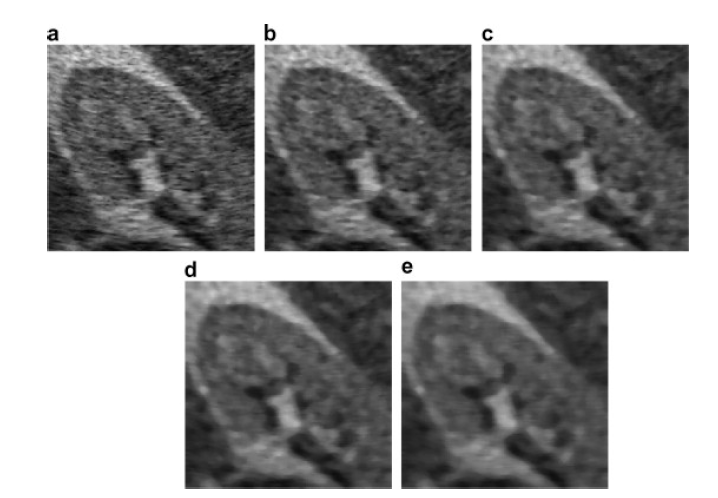
\includegraphics[width = 0.5\textwidth]{figs/speckle.png}
\end{figure}

La calidad de las imágenes varía considerablemente según el dispositivo, la habilidad del operador y la constitución del paciente. Los equipos portátiles suelen producir imágenes de menor calidad. Además, los artefactos como sombras, reverberaciones y efectos de atenuación dificultan la interpretación, por lo que deben detectarse y corregirse durante el procesamiento. Dado que el ultrasonido es una técnica dinámica y en tiempo real, los algoritmos de procesamiento deben ser rápidos y eficientes, equilibrando calidad de mejora y costo computacional.

\section{Microscopía}

La microscopía óptica captura las interacciones de la luz a escala micro o nanométrica, transformadas por sensores digitales en datos de píxeles. Las tareas de procesamiento incluyen corrección de enfoque automático, eliminación de ruido (especialmente en imágenes de fluorescencia con poca luz), y mejora de contraste o iluminación desigual. Los desafíos incluyen la calibración precisa para mantener la resolución espacial, la segmentación de células superpuestas y el manejo de grandes volúmenes de datos generados por la microscopía de alto rendimiento. En este contexto, se aplican métodos de aprendizaje profundo para la segmentación y eliminación de ruido, así como enfoques computacionales avanzados como la reconstrucción holográfica.

Las aplicaciones abarcan el conteo celular, el análisis morfológico, la patología, el cribado de fármacos y la investigación en biología molecular. Dada la variabilidad entre imágenes microscópicas, los pasos de preprocesamiento deben priorizar la corrección de iluminación, la normalización del color y la reducción de ruido antes del análisis cuantitativo.

\section{Integración y flujo de trabajo clínico}

Las modalidades de imagen suelen utilizarse conjuntamente, como en PET/CT o PET/MRI. Los flujos de trabajo automatizados incluyen reducción de ruido, registro y segmentación, apoyándose en estaciones centralizadas de procesamiento de imágenes médicas para la visualización multimodal. El éxito del procesamiento depende de comprender tanto la física de formación de cada modalidad como su contexto clínico.

\section{Conclusión}
\begin{itemize}
\item \textbf{CT:} Modalidad basada en rayos X que genera mapas tridimensionales de densidad. Los principales retos incluyen el ruido, artefactos como endurecimiento del haz o rayas metálicas, y la segmentación de tejidos blandos en presencia de estructuras de alto contraste.

\item \textbf{PET y SPECT:} Técnicas de medicina nuclear que miden la distribución funcional de trazadores. Presentan alto ruido por conteo limitado de fotones, correcciones complejas por atenuación y dispersión, necesidad de registro con CT o MRI, baja resolución y dificultades de análisis cuantitativo.

\item \textbf{Microscopía:} Imagen óptica de tejidos y células a micro/nanoescala, con retos de alta resolución, iluminación desigual, ruido en baja luz, segmentación compleja y grandes volúmenes de datos.

\item \textbf{Ultrasonido:} Imagen en tiempo real basada en ondas sonoras, afectada por ruido de moteado, variabilidad dependiente del operador y el equipo, artefactos de sombra y reverberación, y restricciones de procesamiento en tiempo real.

\end{itemize}
